% Intended LaTeX compiler: xelatex
\documentclass[10pt, svgnames]{beamer}
\usepackage{graphicx}
\usepackage{longtable}
\usepackage{wrapfig}
\usepackage{rotating}
\usepackage[normalem]{ulem}
\usepackage{amsmath}
\usepackage{amssymb}
\usepackage{capt-of}
\usepackage{hyperref}
\usetheme{metropolis}
\author{Sappinandana Akamphon}
\date{\today}
\title{Introduction to Engineering Design}
\subtitle{ME 310: Mechanical Design}
\usepackage{booktabs}
\usepackage{pgfplots}
\usepackage{multirow}
\usepackage{smartdiagram}
\pgfplotsset{compat=1.18}
\institute{Department of Mechanical Engineering, TSE}
\date{}
\usetikzlibrary{patterns,shapes,arrows}
\AtBeginSection[]{\begin{frame}{Outline}\tableofcontents[currentsection]\end{frame}}
\hypersetup{
 pdfauthor={Sappinandana Akamphon},
 pdftitle={Introduction to Engineering Design},
 pdfkeywords={},
 pdfsubject={},
 pdfcreator={Emacs 30.0.50 (Org mode 9.6)}, 
 pdflang={English}}
\begin{document}

\begin{frame}
\maketitle
\end{frame}

\begin{frame}[label={sec:orgf7890b3}]{Who am I?}
Sappinandana Akamphon \\\empty
ENG 421/4 \\\empty
sup@engr.tu.ac.th
\end{frame}

\begin{frame}[label={sec:orgfa8bff3}]{What are we covering?}
\begin{itemize}
\item Design principles
\item Power sources and transmission
\item Joints
\item Power transmission components
\end{itemize}
\end{frame}

\begin{frame}[label={sec:org99f5de2}]{Expected Skills at the End}
Analyze and design a simple mechanical power transmission system
\end{frame}

\begin{frame}[label={sec:orgc56ffbb}]{Schedule}
\small
\begin{center}
  \begin{tabular}{rl}
    \hline
    \toprule
    Week & \multicolumn{1}{c}{Topics} \\
    \midrule
    1 & Engineering Design Processes. Safety Factors. \\
    2 & Review of Mechanics of Materials. Stress Concentration. \\
    3 & Materials Selection. \\
    4 & Shafts and Shaft Components. \\
    5 & Mechanical Springs. \\
    6 & Welding, Bonding, Permanent Joints. \\
    7 & Screws, Fasteners, Nonpermanent Joints. \\
    8 & \textbf{Midterm} \\
    9 & Rolling-Contact Bearings. \\
    10 & Lubrication and Journal Bearings. \\
    11 & Spur and Helical Gears. \\
    12 & Bevel and Worm Gears. \\
    13 & Clutches, Brakes, and Couplings. \\
    14 & Belts, Chains, and Ropes. \\
    15 & Case Studies \\
    \bottomrule
  \end{tabular}
\end{center}
\end{frame}

\begin{frame}[label={sec:org5ba24aa}]{Reading Materials}
\begin{itemize}
\item Akamphon. S., 2020, ME 310: Mechanical Design I.

\item Juvinall, R. C., and Marshek, K. M., 2006, Fundamentals of Machine
Component Design. 4th Edition, Wiley.

\item Hibbeler, R. C., 1997, Mechanics of Materials, 3rd Edition, Prentice
Hall.

\item Shigley, J. E. and C. R. Mischke, 2009, Mechanical Engineering Design.
McGraw Hill.
\end{itemize}
\end{frame}

\begin{frame}[label={sec:org904268d}]{Grading}
\begin{center}
  \begin{tabular}{ll}
    \toprule
    Project I progress & 10\% \\
    Project I & 10\% \\
    Midterm & 30\% \\
    Project II progress & 10\% \\
    Project II & 10\% \\
    Final & 30\% \\
    \bottomrule
  \end{tabular}
\end{center}
\end{frame}

\begin{frame}[label={sec:orgd911876}]{Engineering Design}
\begin{itemize}
\item Application of science and engineering
\item Define structure of system in details
\item Allow manufacturers to be able to make it
\end{itemize}
\end{frame}

\begin{frame}[label={sec:org5714a6d}]{What about Mechanical Design?}
Mechanical engineers need to define

\begin{itemize}
\item Materials
\item Dimensions
\item Shapes
\end{itemize}

So that the designed product can function properly
\end{frame}

\begin{frame}[label={sec:orgdcb13cd}]{Engineering Design Processes}
\begin{center}
\smartdiagram[circular diagram:clockwise]{Ask, Research, Imagine, Plan, Create, Test, Improve}
\end{center}
\end{frame}

\begin{frame}[label={sec:orgc5c3a14}]{Ask: What seems to be the problem?}
\begin{itemize}
\item What do you want to make?
\item Why is it needed?
\item What is the product supposed to do/not to do?
\end{itemize}
\end{frame}

\begin{frame}[label={sec:orgc8a640c}]{Research: More details on the problems and products}
\begin{itemize}
\item Talk to customers to better understand problems and needs
\item Conduct independent research get a clearer picture
\item Look into previous works/products. What works? What doesn't?
\end{itemize}
\end{frame}

\begin{frame}[label={sec:org94dfeab}]{Imagine: Come up with conceptual design}
\begin{itemize}
\item Brainstorm ideas
\item Exchange opinions on different solutions
\end{itemize}
\end{frame}

\begin{frame}[label={sec:org484b076}]{Plan: How should we proceed?}
\begin{itemize}
\item Check problems, needs, constrains
\item Evaluate ideas and select the best one
\item Plan how to move forward
\end{itemize}
\end{frame}

\begin{frame}[label={sec:org0af7674}]{Create: Make it happen}
\begin{itemize}
\item Design the components
\item Respect constraints and requirements developed earlier
\item Build prototype and verify
\end{itemize}
\end{frame}


\begin{frame}[label={sec:orgae05472}]{Test: Does it work?}
\begin{itemize}
\item Perform analysis and test on prototype
\item Use in actual operating conditions
\item Get feed back from customers
\item Evaluate what needs improvement
\end{itemize}
\end{frame}


\begin{frame}[label={sec:org9c1441b}]{Improve: Make it better}
\begin{itemize}
\item Redesign and improve based on feedback and tests
\end{itemize}
\end{frame}


\begin{frame}[label={sec:org68343ad}]{Application of Engineering Design: Lawn Mower}
\begin{itemize}
\item So many lawn in Thammasat
\item How do you keep them all nice and tidy?
\end{itemize}
\end{frame}


\begin{frame}[label={sec:orgef20b7f}]{Scisscors?}
\begin{center}
  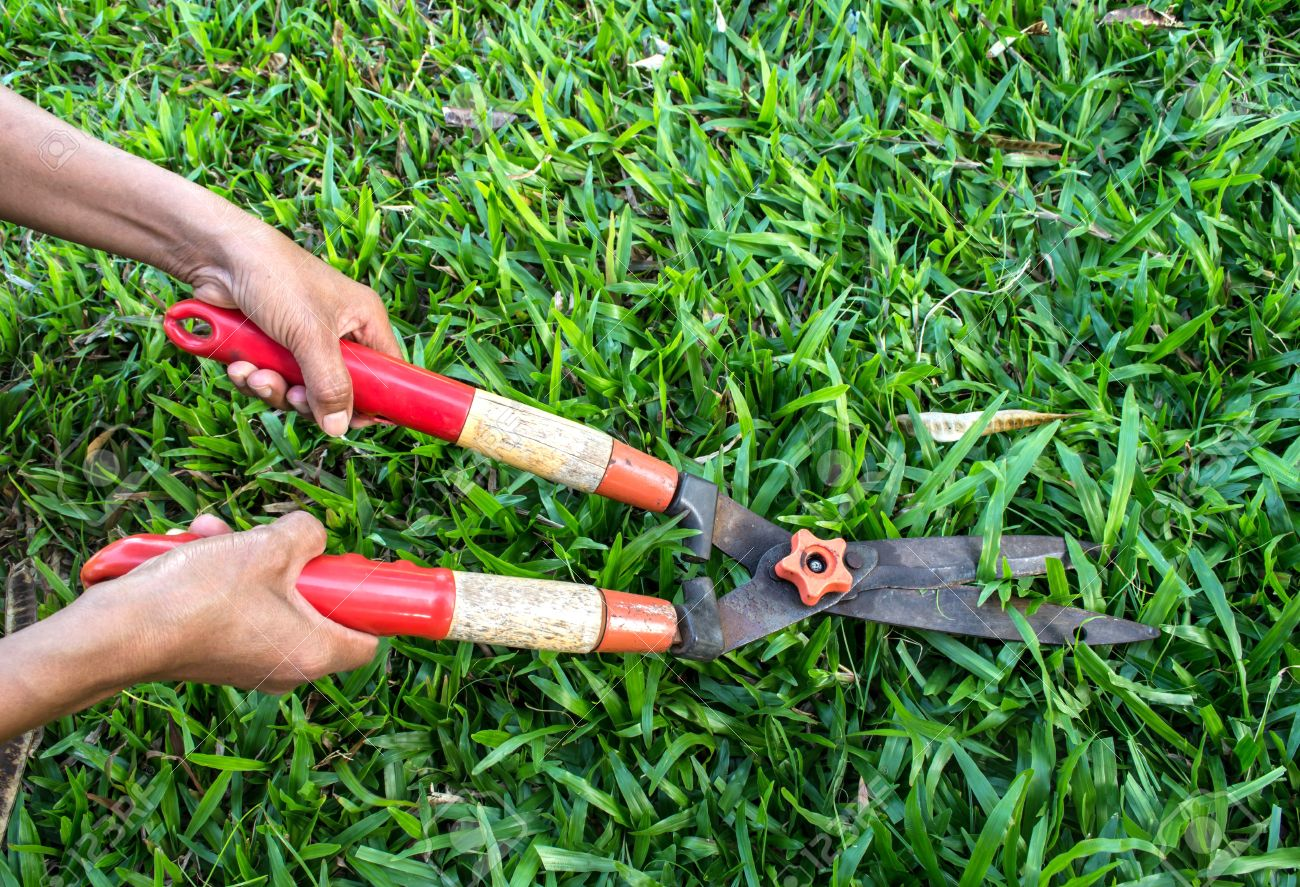
\includegraphics[width=.9\linewidth]{./pictures/grass-shears.jpg}
\end{center}
\end{frame}

\begin{frame}[label={sec:org7aae4db}]{Machete?}
\begin{center}
  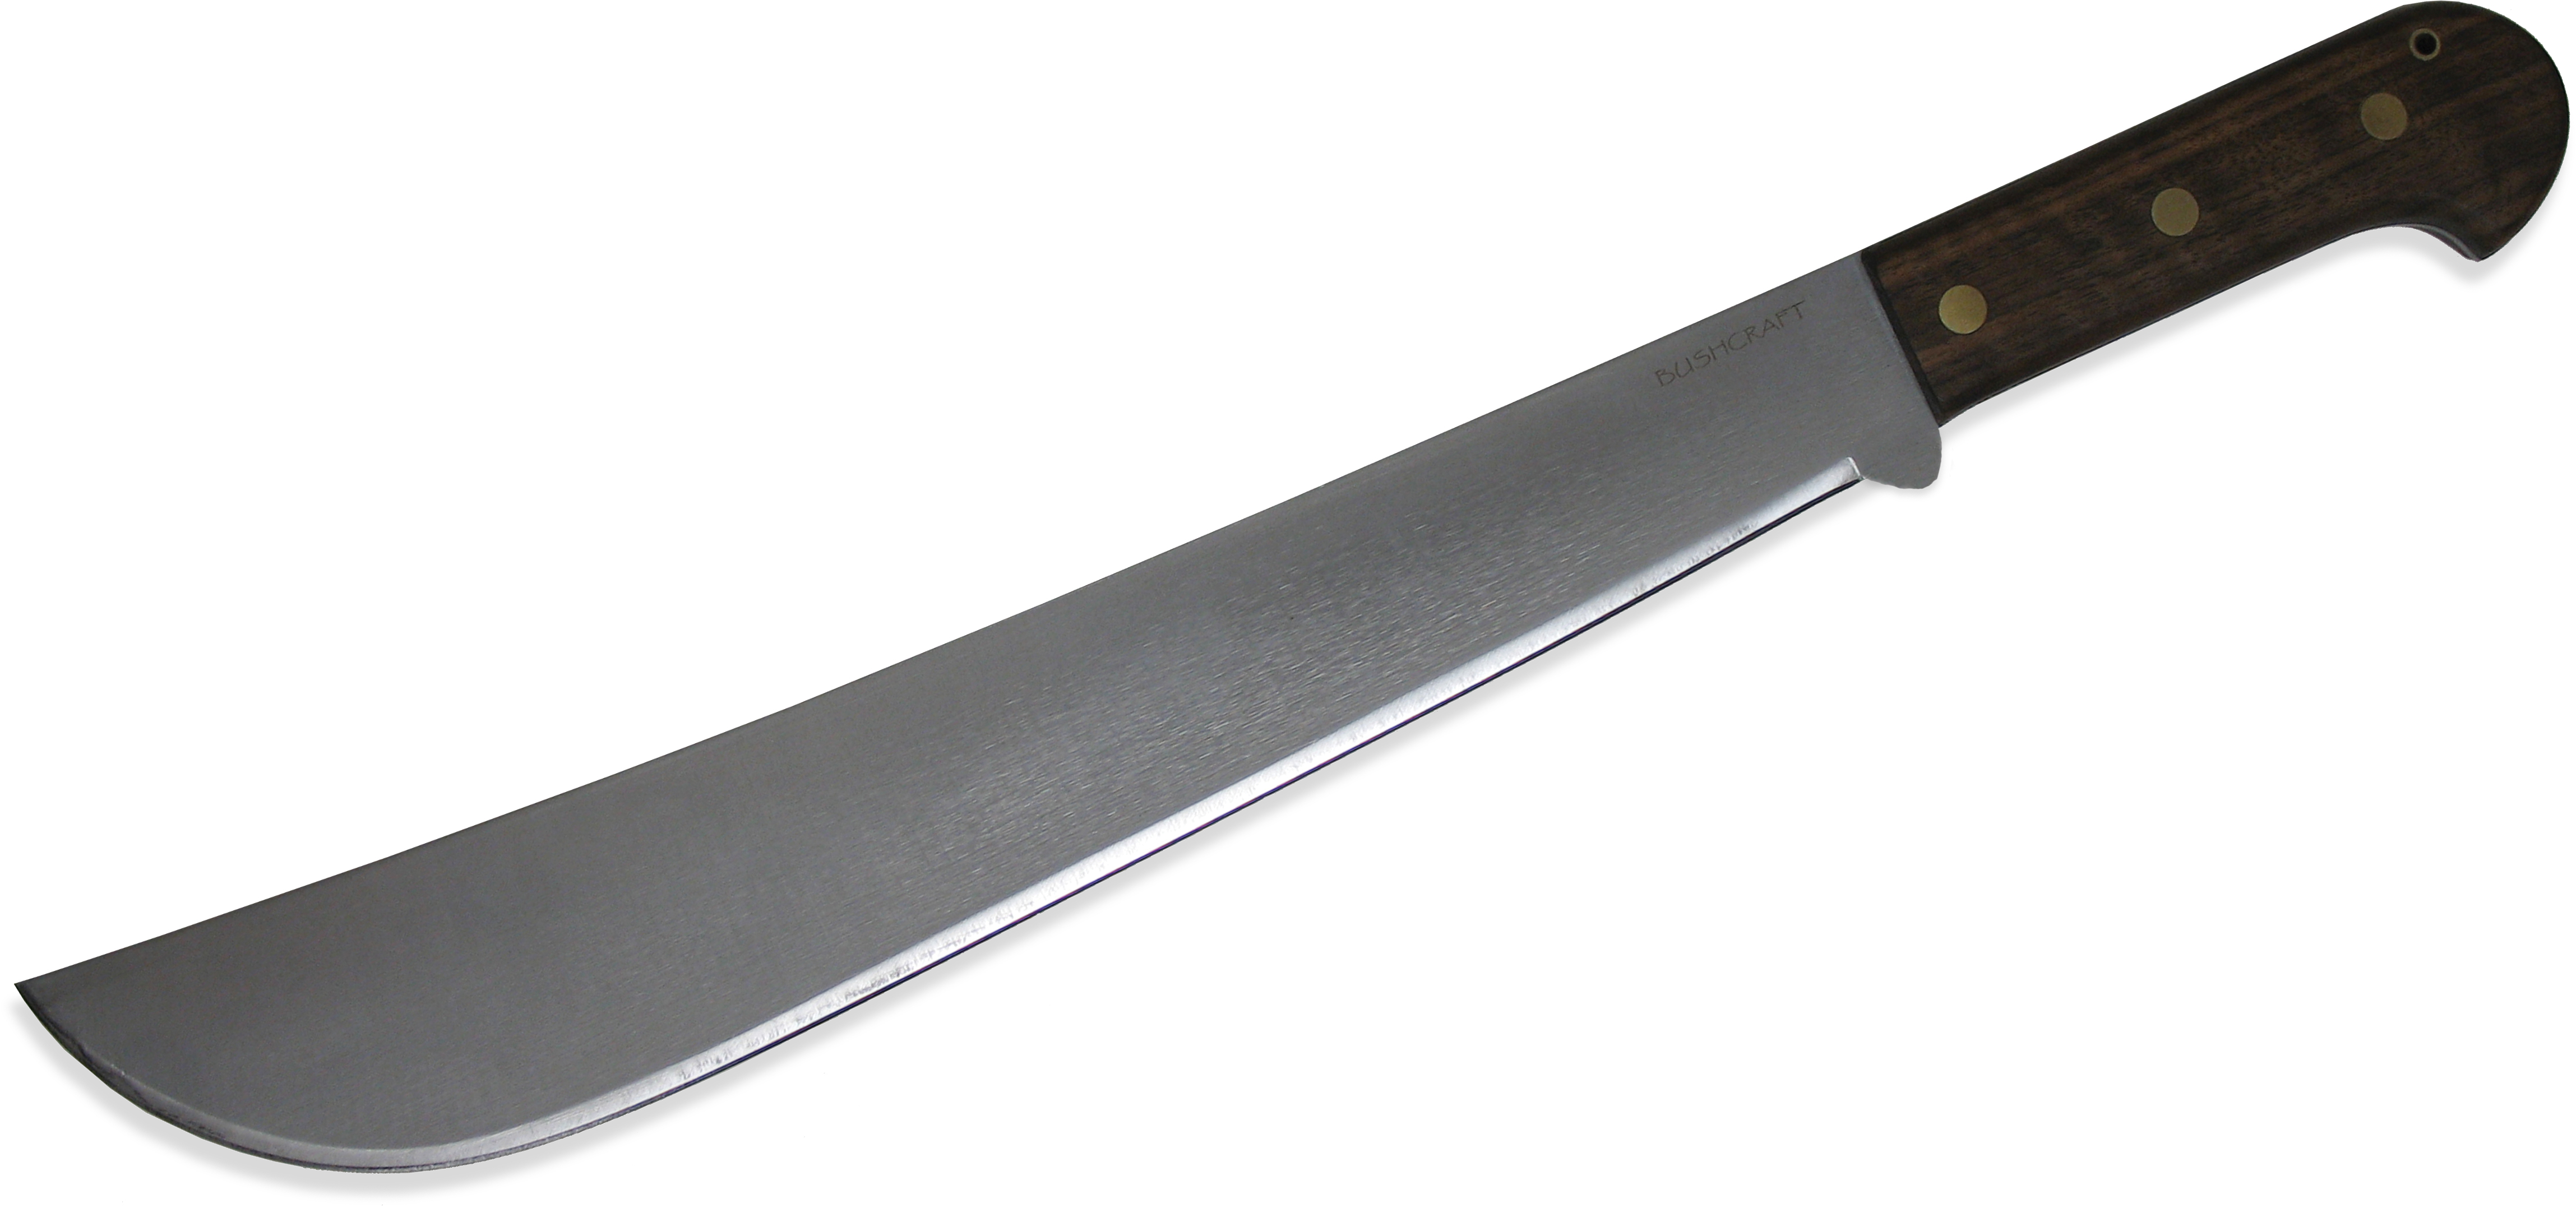
\includegraphics[width=.9\linewidth]{./pictures/machete.jpg}
\end{center}
\end{frame}

\begin{frame}[label={sec:org96aafce}]{Lawn Mower?}
\begin{center}
  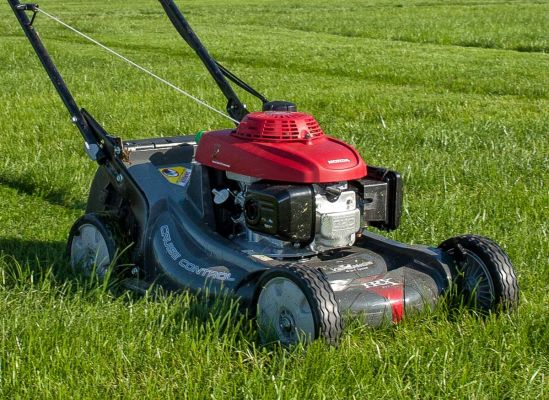
\includegraphics[width=.9\linewidth]{./pictures/lawn-mower.jpg}
\end{center}
\end{frame}

\begin{frame}[label={sec:org9c0ef32}]{Case Study: Grass Cutting Solution}
\begin{itemize}
\item Lawn Mowers \(\rightarrow\) fast, but cumbersome
\item Shears/Machete \(\rightarrow\) slow, portable
\end{itemize}


\begin{figure}[h]
  \centering
  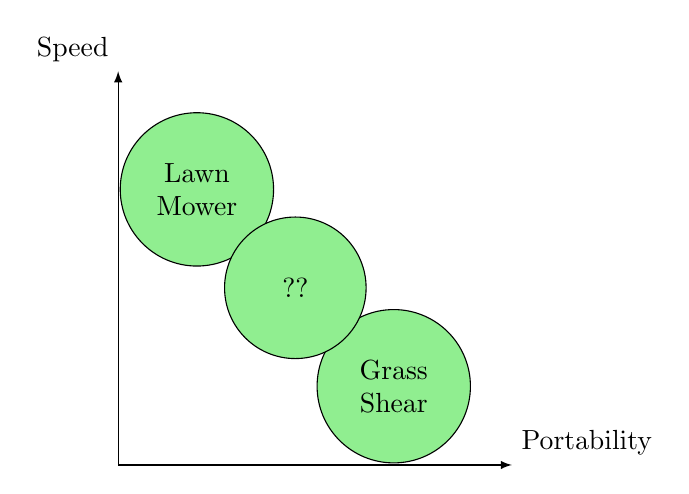
\begin{tikzpicture}[>=latex]
    \draw[->] (0,0) --++ (90:5) node[above left]{Speed};
    \draw[->] (0,0) --++ (0:5) node[above right]{Portability};
    \node at (1,3.5) [draw, circle, fill=LightGreen, minimum width=1.5cm, text width=1.5cm, align=center]{Lawn Mower};
    \node at (3.5,1) [draw, circle, fill=LightGreen, minimum width=1.5cm, text width=1.5cm, align=center]{Grass Shear};
    \node at (2.25,2.25) [draw, circle, fill=LightGreen, minimum width=1.5cm, text width=1.5cm, align=center]{??};
  \end{tikzpicture}
\end{figure}
\end{frame}

\begin{frame}[label={sec:org5b4c89d}]{Can we do any better? Something in between?}
\begin{itemize}
\item Make one yourself
\end{itemize}
\end{frame}


\begin{frame}[label={sec:orgeb5501c}]{Defining Key Component}
\begin{itemize}
\item What is the most important component in a grass cutting device?
\item A component that completes the main function
\item For a grass-cutter device \(\rightarrow\) the cutting mechanism
\end{itemize}
\end{frame}


\begin{frame}[label={sec:org1352485}]{The cutting mechanism\ldots{} obviously}
\begin{itemize}
\item blade, shear, \ldots{}
\end{itemize}

\begin{center}
  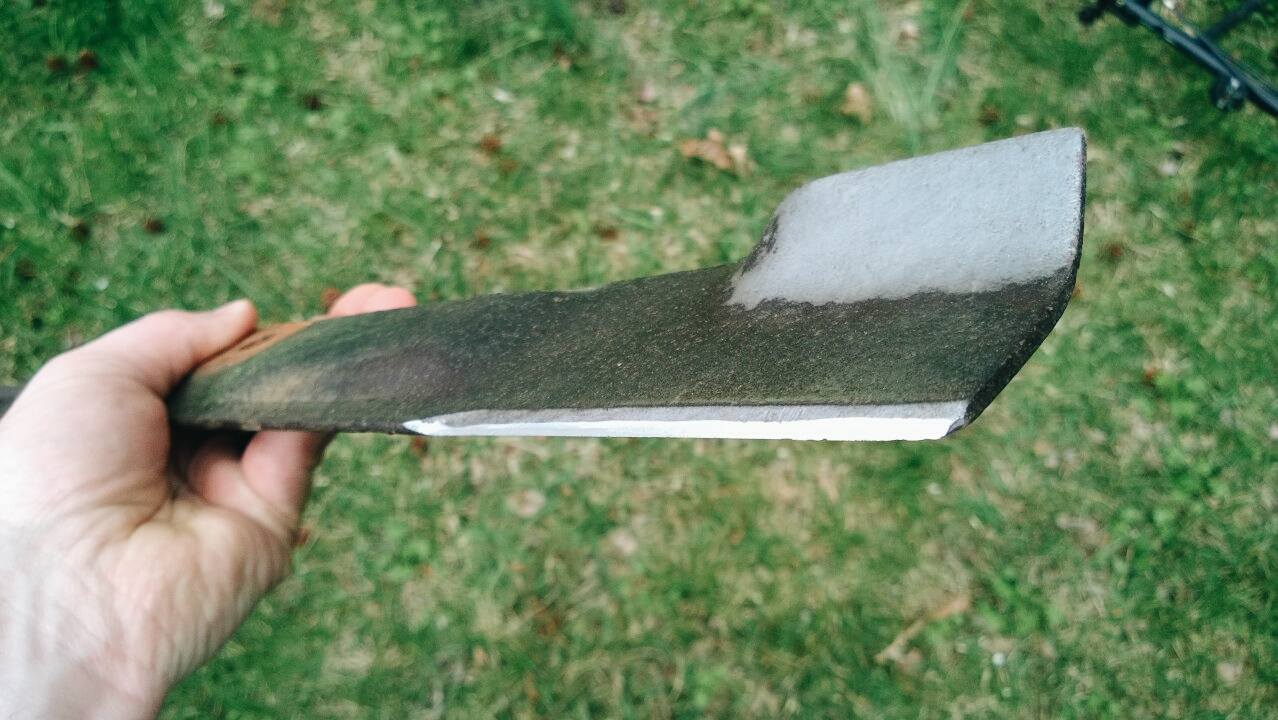
\includegraphics[width=.9\linewidth]{./pictures/mower-blade.jpg}
\end{center}
\end{frame}

\begin{frame}[label={sec:orgd2bd6fd}]{Key Analysis: Shearing Force}
\begin{center}
  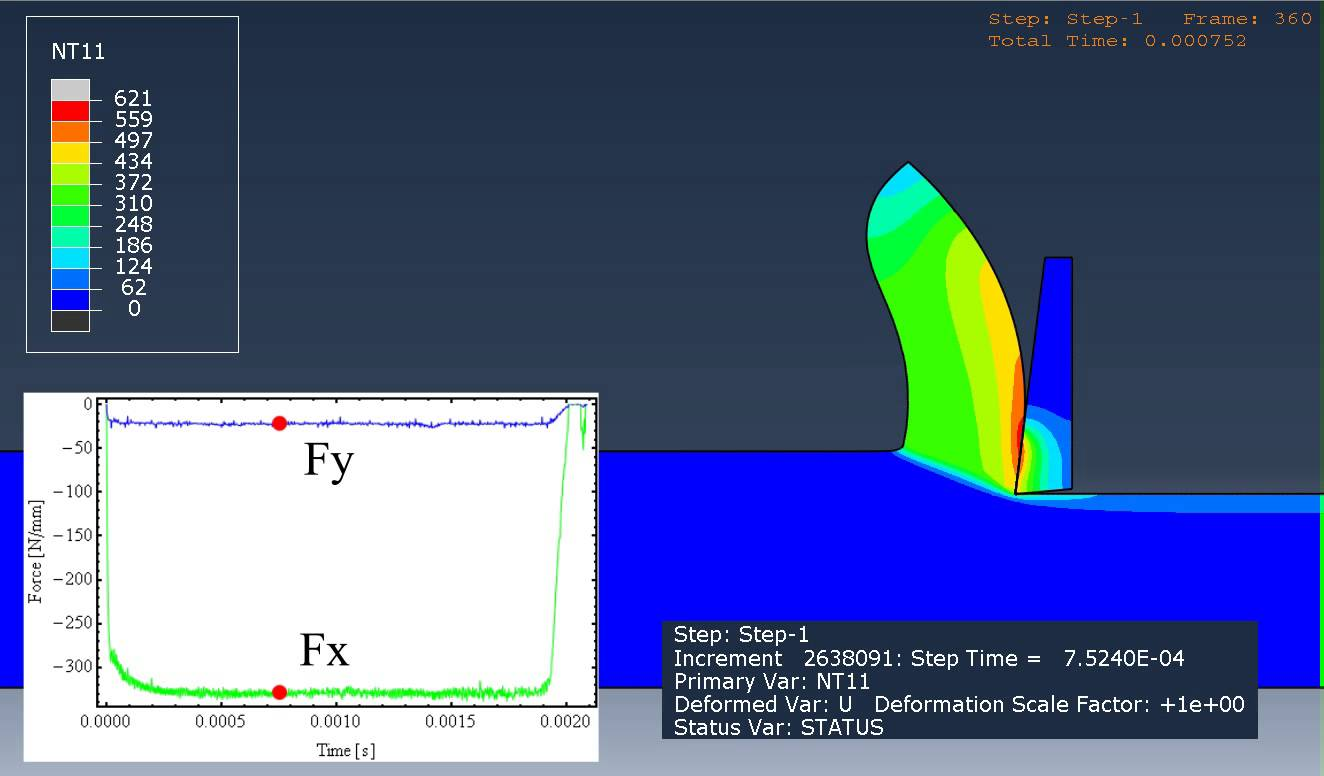
\includegraphics[width=.9\linewidth]{./pictures/cutting.jpg}
\end{center}
\end{frame}

\begin{frame}[label={sec:org883cc3a}]{Same problem, different approach}
\begin{itemize}
\item blade \(\rightarrow\) hard, sharp, but moving slowly
\item can something softer, but moving fast does the same job?
\end{itemize}
\end{frame}


\begin{frame}[label={sec:org0132e99}]{Fast spinning wires?}
\begin{center}
  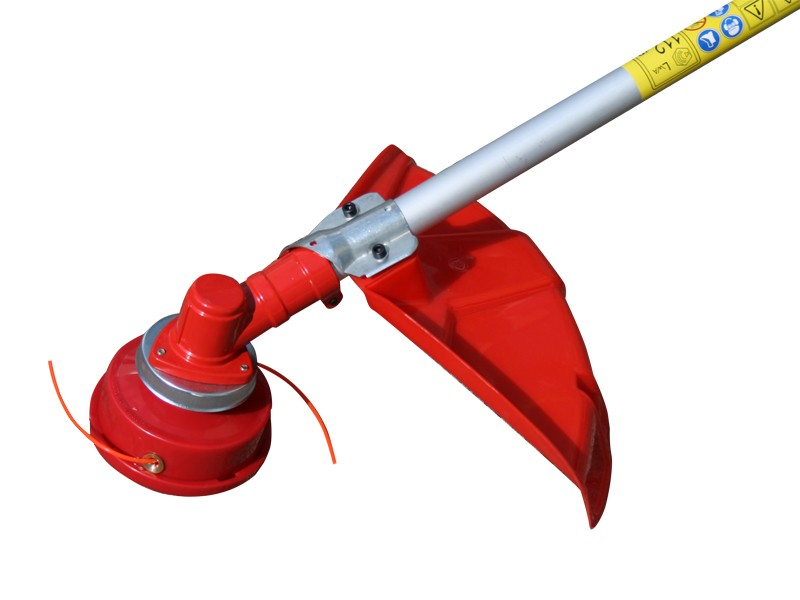
\includegraphics[width=.8\linewidth]{./pictures/cutter-wire.jpg}
\end{center}
\end{frame}

\begin{frame}[label={sec:org2f8750e}]{Problem \(\rightarrow\) Component}
\begin{itemize}
\item Define what needs to be done
\item Be specific
\item Most design problems already have partial solutions
\end{itemize}
\end{frame}


\begin{frame}[label={sec:orgd744ef4}]{Defining constraints}
\begin{itemize}
\item Deadline?
\item Budget?
\item Load requirements?
\end{itemize}
\end{frame}


\begin{frame}[label={sec:orgd043141}]{Finding best solution}
\begin{itemize}
\item Systematic method
\item Validate \& evaluate possible solutions
\end{itemize}
\end{frame}


\begin{frame}[label={sec:orgf7e989d}]{FRDPARRC Chart}
\begin{description}
\item[{FR}] Functional Requirements \(\rightarrow\) what job does it have?
\item[{DP}] Design Parameters \(\rightarrow\)  what dimensions/shapes/materials does the job?
\item[{A}] Analysis \(\rightarrow\) how would you determine that proper DP?
\item[{R}] References \(\rightarrow\) where do you get that method(s) from?
\item[{R}] Risks \(\rightarrow\) is there any potential problems from your design?
\item[{C}] Countermeasures \(\rightarrow\) how do you solve that potential problem?
\end{description}
\end{frame}

\begin{frame}[label={sec:org7fc16bf}]{Case Study: Coconut Milk Production}
\begin{columns}
  \begin{column}{0.5\columnwidth}
    \begin{center}
      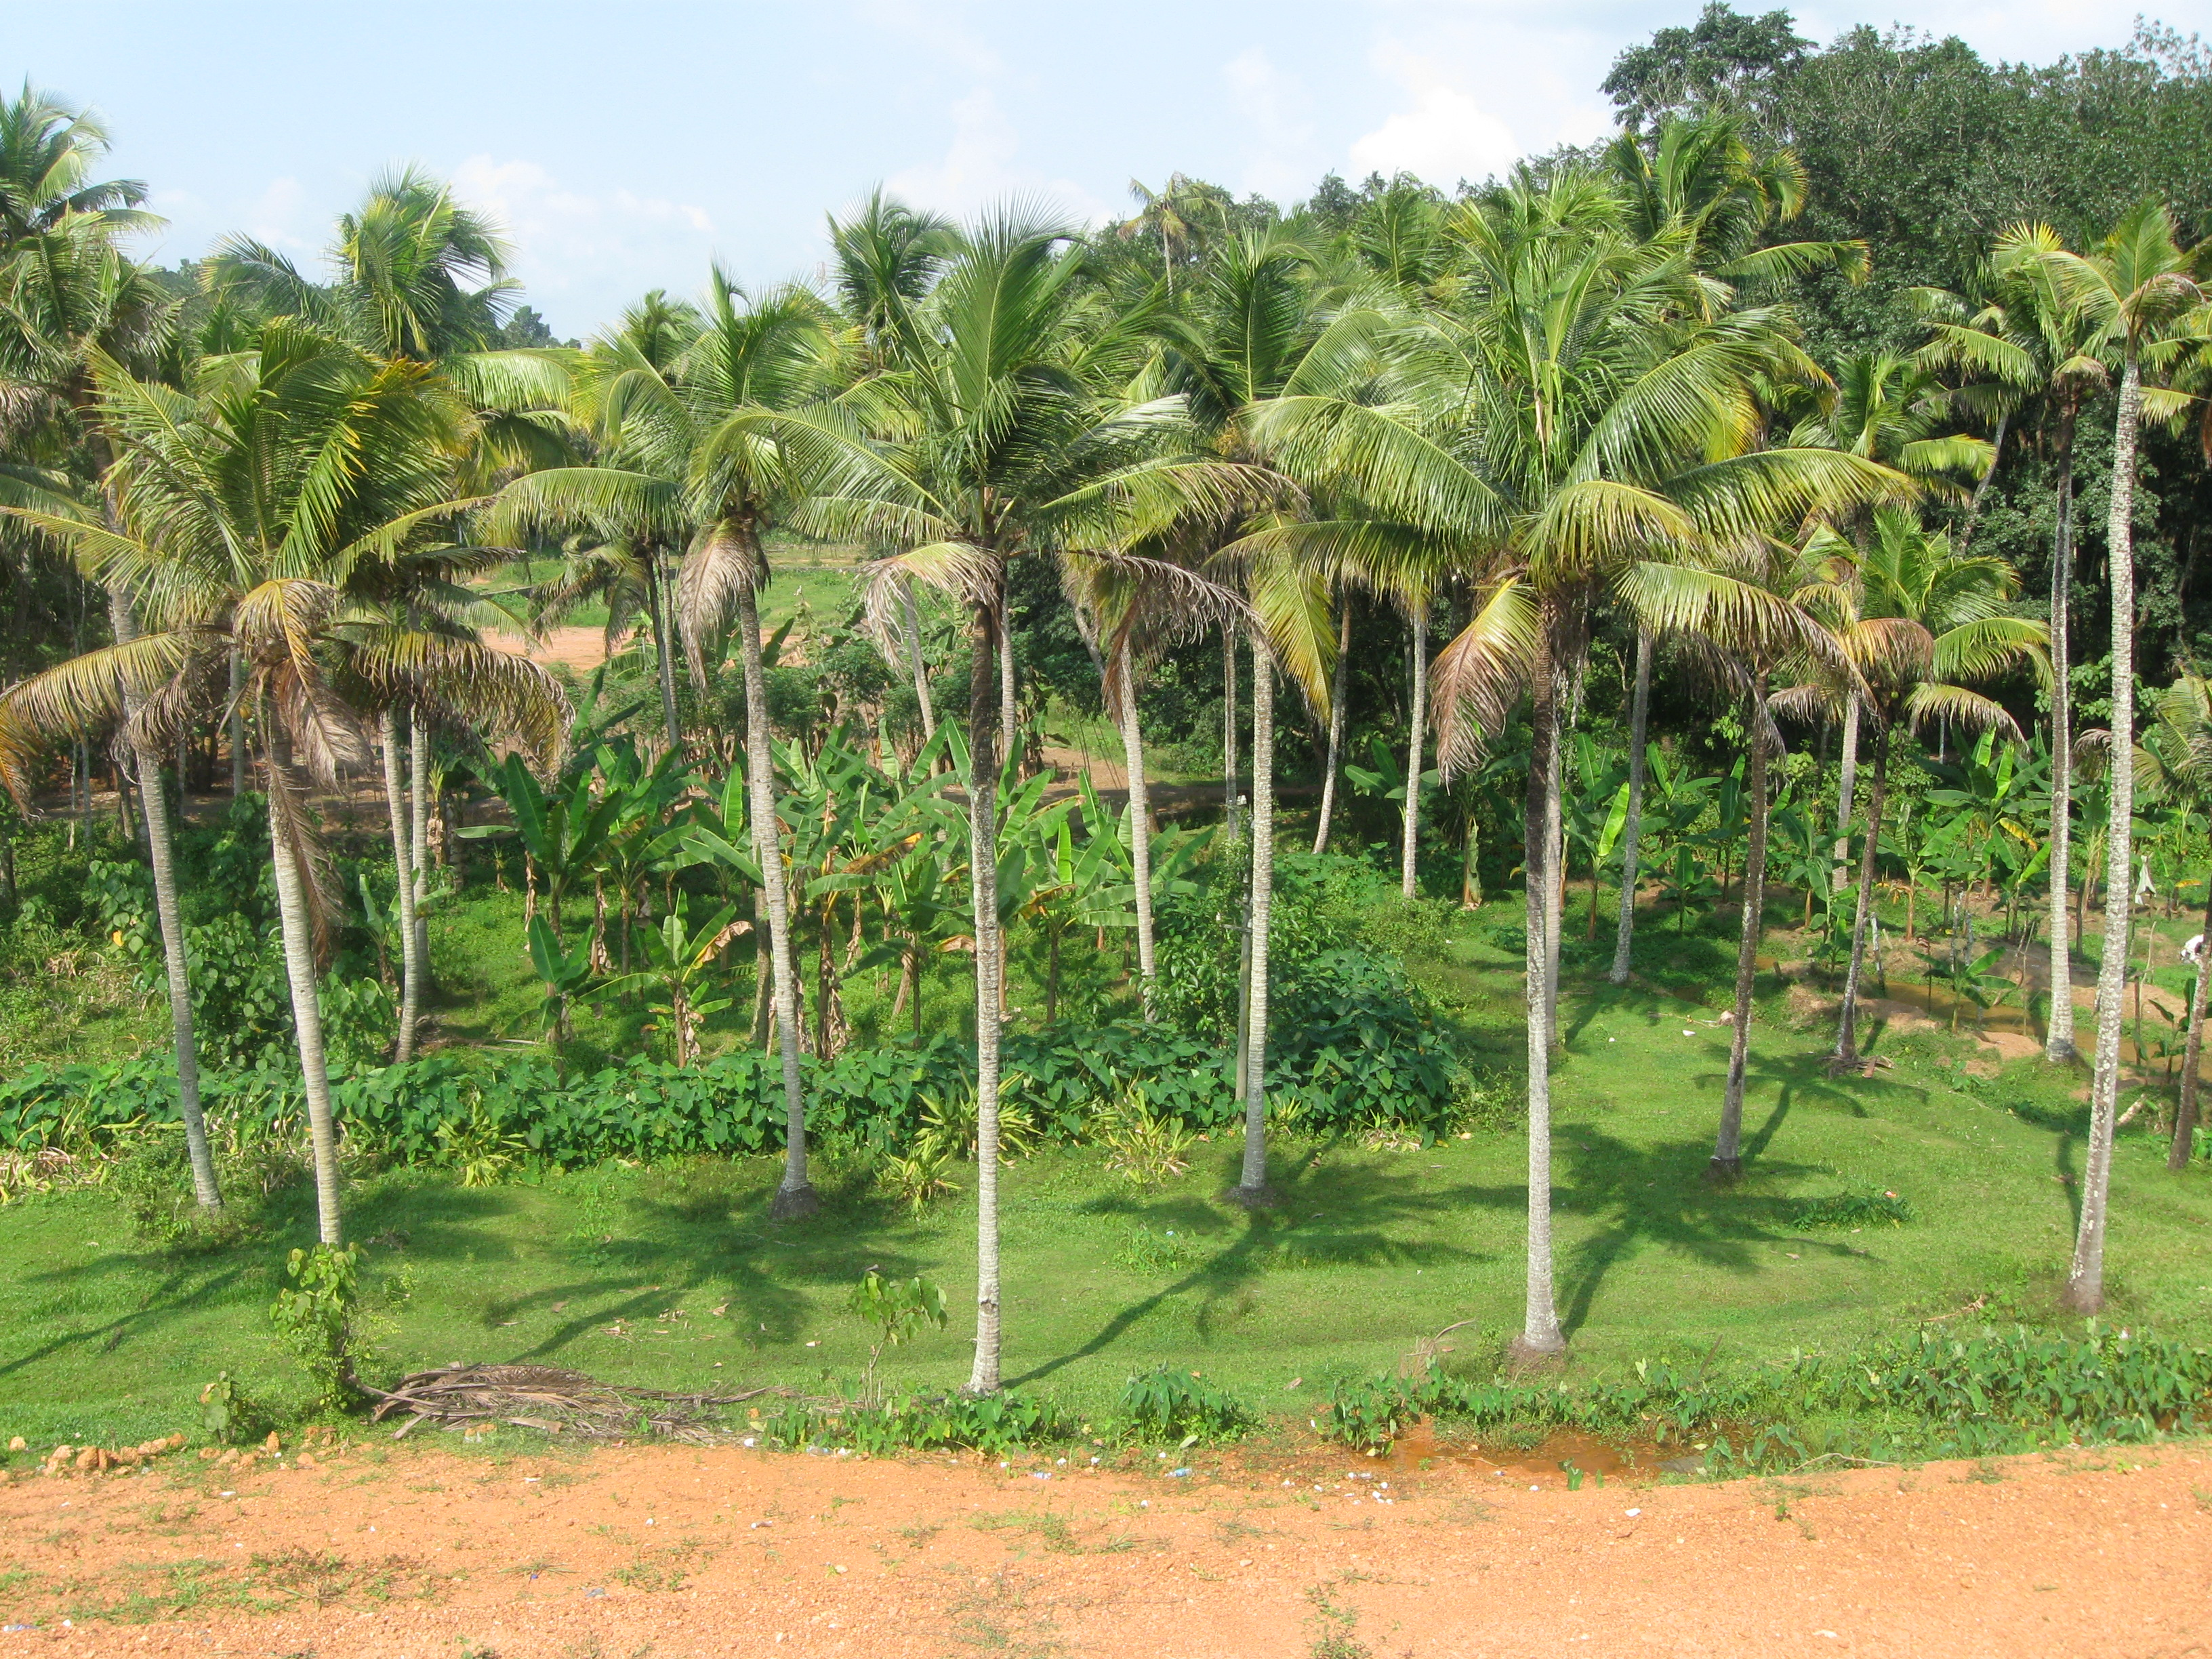
\includegraphics[width=.9\linewidth]{./pictures/coconut-orchard.JPG}
    \end{center}
  \end{column}

  \begin{column}{0.5\columnwidth}
    \begin{center}
      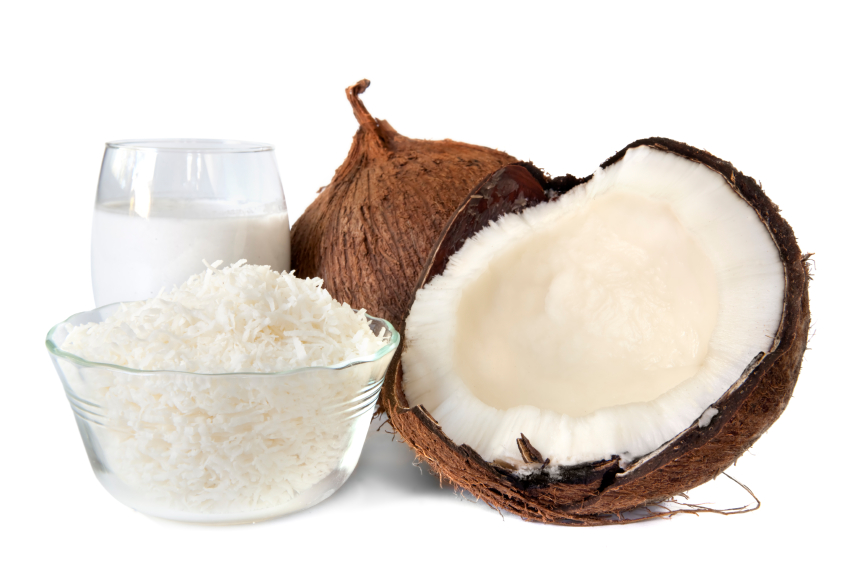
\includegraphics[width=.9\linewidth]{./pictures/coconut-milk.jpg}
    \end{center}
  \end{column}
\end{columns}
\end{frame}

\begin{frame}[label={sec:org1357d81}]{Current solution: coconut rabbit!?}
\begin{columns}
  \begin{column}{0.45\columnwidth}
    \begin{center}
      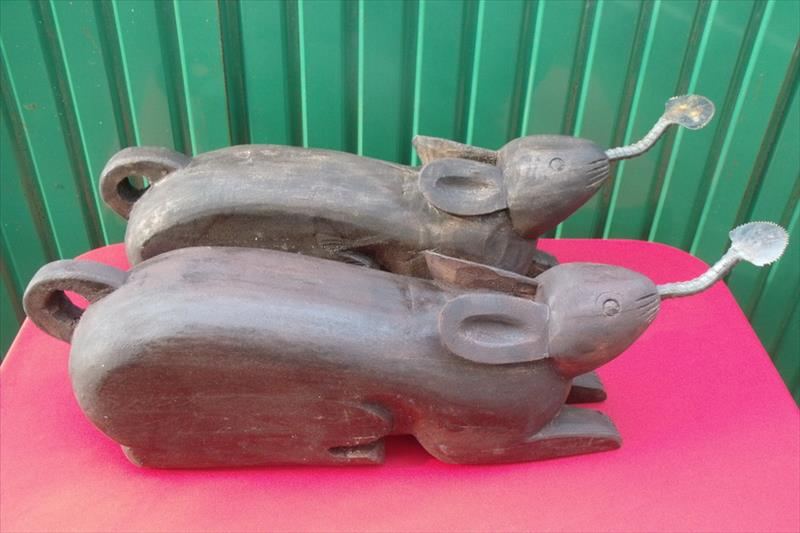
\includegraphics[width=\linewidth]{./pictures/coconut-rabbit.jpg}
    \end{center} 
  \end{column}

  \begin{column}{0.45\columnwidth}
    \begin{center}
      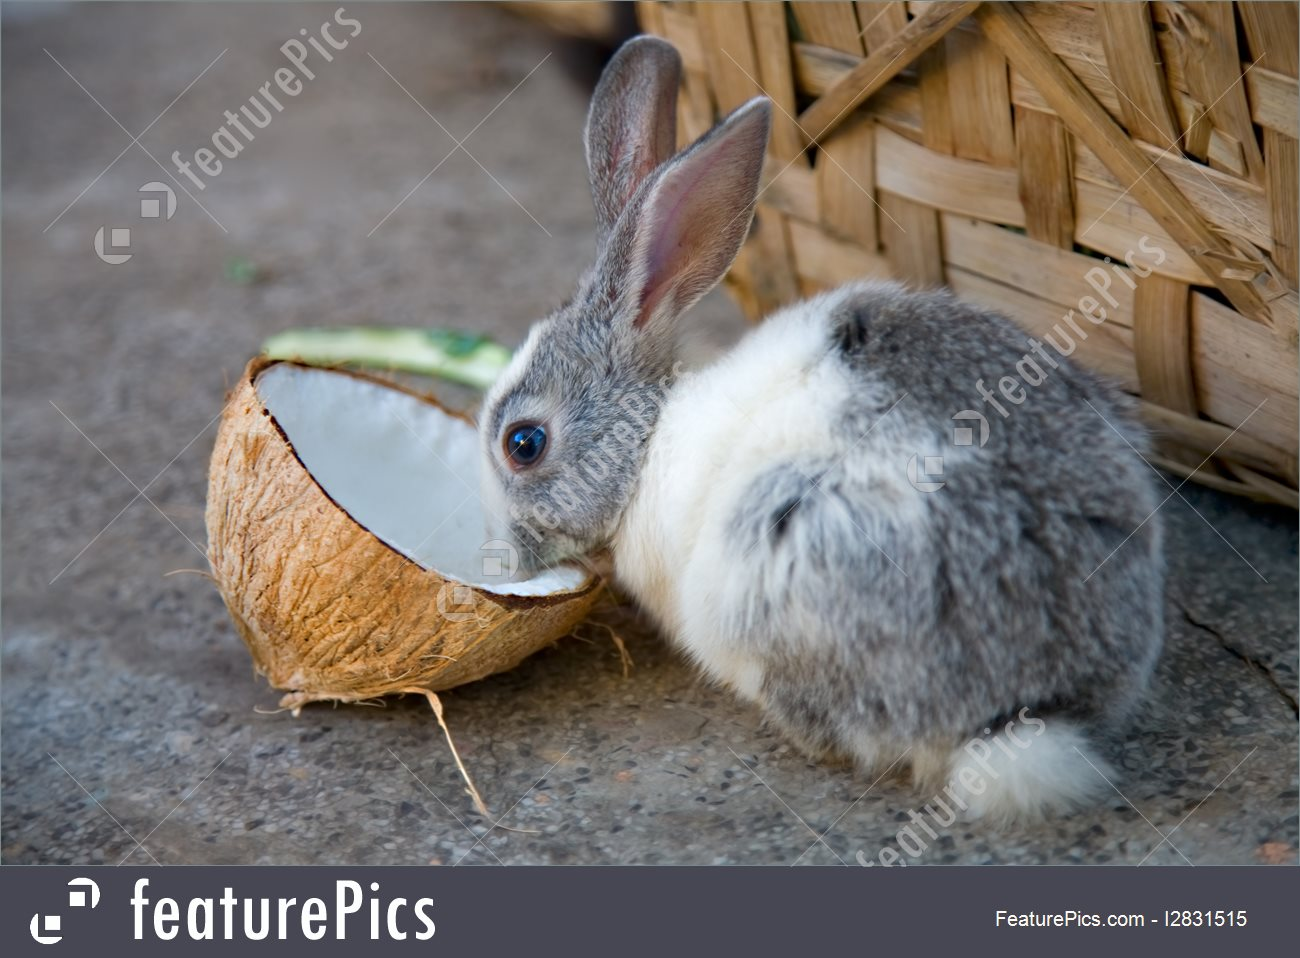
\includegraphics[width=\linewidth]{./pictures/rabbit-eating-coconut.jpg}
    \end{center}
  \end{column}
\end{columns}
\end{frame}



\begin{frame}[label={sec:org3a9e25c}]{Develop idea through FRDPARRC chart}
\begin{itemize}
\item Goal: obtain scraped/minced coconut meat for squeezing into coconut milk
\end{itemize}

\begin{center}
  \begin{tabular}{lll}
    \hline
    FR & Scrape meat & Pulverize meat + shell\\
    \hline
    DP & Scraper & Grinder\\
    \hline
    A & Strength of meat & Strength of shell + meat\\
       & Beam bending & Grinding teeth strength\\
    \hline
    R & Mechanics of Materials & Mechanics of Materials\\
       & Statics & Statics\\
    \hline
    R & Scraper teeth broken & Stuck grinder\\
    \hline
    C & Additional focus on teeth strength & Check clearance\\
    \hline
  \end{tabular}
\end{center}
\end{frame}

\begin{frame}[label={sec:org58d81fd}]{Final Products}
\begin{columns}
  \begin{column}{0.5\columnwidth}
    \begin{center}
      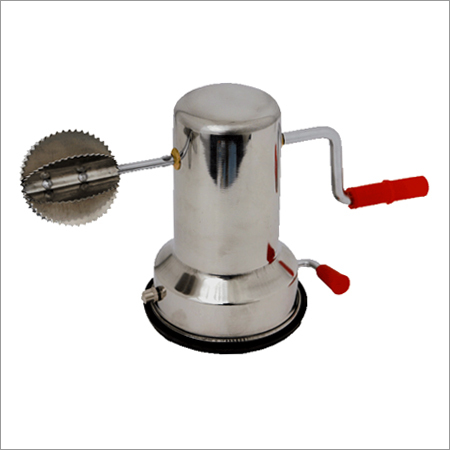
\includegraphics[width=.9\linewidth]{./pictures/coconut-scraper.png}
    \end{center}
  \end{column}

  \begin{column}{0.5\columnwidth}
    \begin{center}
      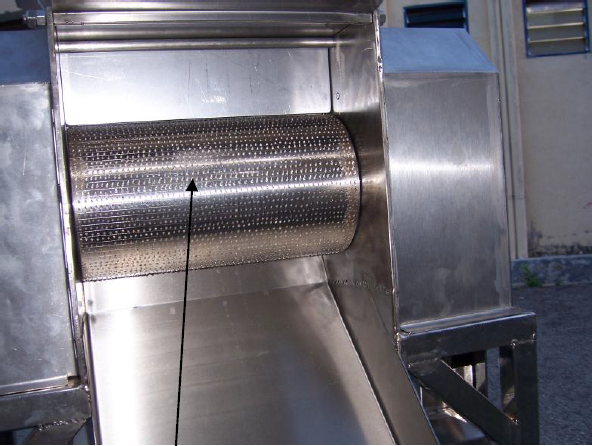
\includegraphics[width=.9\linewidth]{./pictures/coconut-grinder.png}
    \end{center}
  \end{column}
\end{columns}
\end{frame}

\begin{frame}[label={sec:org75ab8f1}]{Major Design Considerations}
\begin{itemize}
\item Strength
\item Deformation
\item Uncertainty
\end{itemize}
\end{frame}


\begin{frame}[label={sec:org878b34d}]{Strength vs Stress}
\begin{center}
  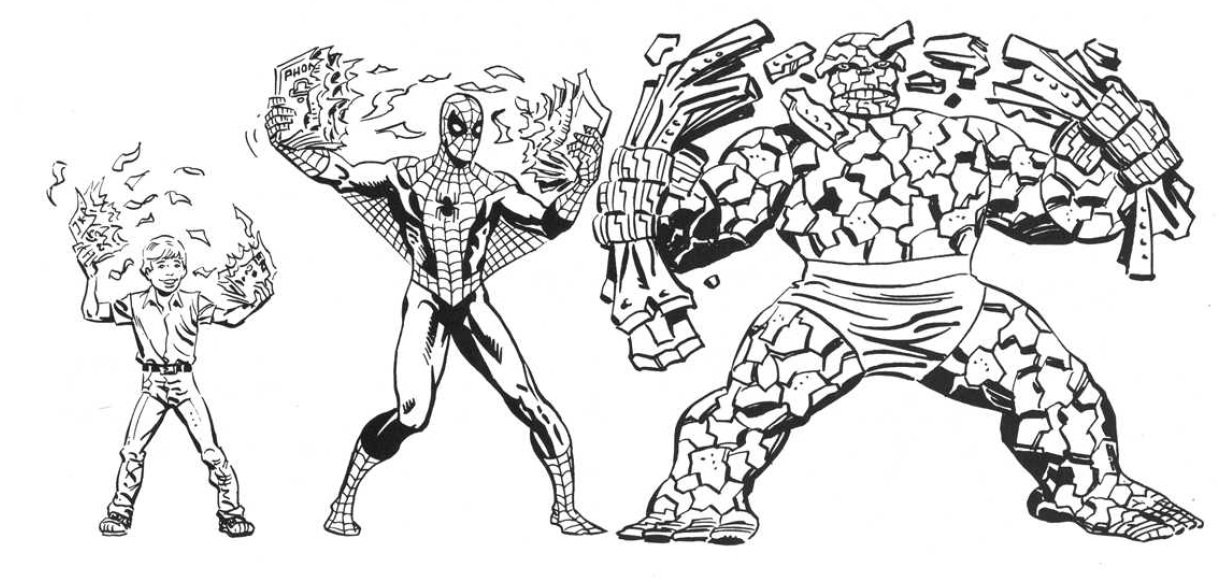
\includegraphics[width=.9\linewidth]{./pictures/strength-stress.jpg}
\end{center}
\begin{equation*}
  strength < stress \rightarrow failure
\end{equation*}
\end{frame}

\begin{frame}[label={sec:org884c0f9}]{Deformation}
\begin{center}
  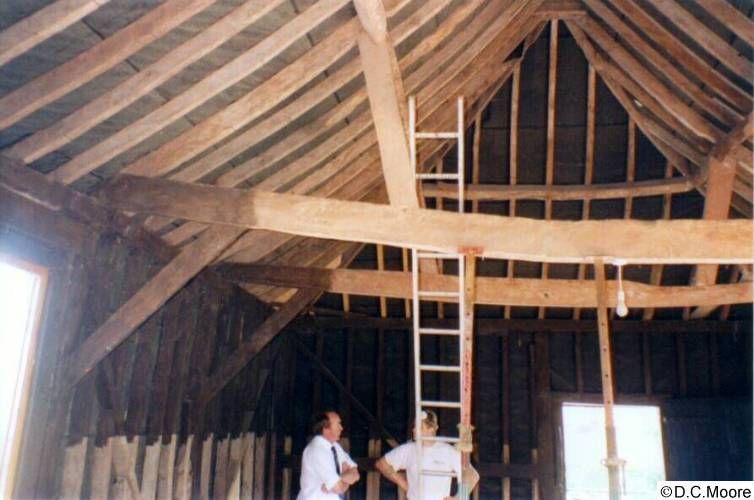
\includegraphics[width=.9\linewidth]{./pictures/deformed-beam.jpg}
\end{center}
\end{frame}

\begin{frame}[label={sec:org703e230}]{How sure are you about \ldots{}}
\begin{itemize}
\item your design calculation(s)?
\end{itemize}


\begin{itemize}
\item your supplier specifications?
\end{itemize}


\begin{itemize}
\item your customer knowledge?
\end{itemize}


\begin{center}
  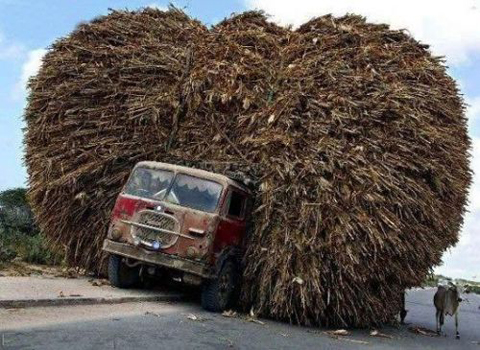
\includegraphics[width=0.7\textwidth]{./pictures/overloaded-truck.jpg}
\end{center}
\end{frame}

\begin{frame}[label={sec:org3bd6746}]{Safety Factor!}
\alert{What is that?}
\end{frame}

\begin{frame}[label={sec:org72bf0b6}]{Safety Factor}
Component should be stronger than the required stress


\begin{itemize}
\item The stronger, the safer it is
\end{itemize}

$$ N_s = \frac{\text{Strength}}{\text{Stress}} $$
\begin{itemize}
\item ``Strength'' and ``Stress'' depend on material and criterion in consideration
\end{itemize}
\end{frame}


\begin{frame}[label={sec:org6cf90de}]{The Safer, The Better \ldots right?}
The bigger safety factor, the safer your component is

So why don't we design everything with a N\(_{\text{s}}\) = 100000
\end{frame}

\begin{frame}[label={sec:org936e18a}]{Too Much of a Good Thing}
Is there a cost for \emph{excessive} safety factor?
\end{frame}

\begin{frame}[label={sec:org9832b0d}]{Total Safety Factor}
\begin{itemize}
\item A choice of safety factor is a combination of mainly two considerations

\begin{itemize}
\item design and usage conditions: how \underline{well} something should be design and manufactured and how \underline{badly} it will be treated.
\item economic and safety factors: how bad it is going to be when it fails.
\end{itemize}
\end{itemize}



\begin{align*}
 N_s = N_{s, cond} N_{s, econ}
\end{align*}
\end{frame}

\begin{frame}[label={sec:org76e030d}]{Design and Condition Safety Factors, \(N_{s,cond}\)}
\begin{center}
  \small
  \begin{tabular}{ll}
    \toprule
    Reliable materials, controllable & 1.25 - 1.5\\
    conditions + loading & \\
    \midrule
    Well-known materials, reasonable & 1.5 - 2\\
    conditions + loading & \\
    \midrule
    Average materials, ordinary & 2 - 2.5\\
    conditions + loading & \\
    \midrule
    Lesser-known materials, average & 2.5 - 3\\
    conditions + loading & \\
    \midrule
    Untried materials + average conditions & \\
    Average materials + unknown conditions & 3 - 4\\
    \midrule
    Repeated loading & use \(S_e\)\\
    \midrule
    Impact forces & Include impact factor\\
    \midrule
    Brittle material (based on \(S_{ut}\)) & Double \(N_s\)\\
    \bottomrule
  \end{tabular}
\end{center}
\end{frame}

\begin{frame}[label={sec:org5cdc3f6}]{Economic and Safety Safety Factors, \(N_{s,econ}\)}
\begin{table}[h]
  \centering
  \begin{tabular}{llccc}
    \toprule
    \multicolumn{2}{l}{\multirow{2}{2.5cm}{Characteristics}} & \multicolumn{3}{c}{Danger to Personnel} \\
    \cmidrule{3-5}
                                                           &          & mild & moderate & severe \\
    \midrule
    \multirow{3}{3cm}{Economic Impact} & mild     & 1.0  & 1.2      & 1.4    \\
                                                           & moderate & 1.0  & 1.3      & 1.5    \\
                                                           & severe   & 1.2  & 1.4      & 1.6    \\
    \bottomrule
  \end{tabular}
\end{table}
\end{frame}

\begin{frame}[label={sec:org8cb81f1}]{Exercise: Design of a Swing Set}
\begin{columns}
\begin{column}{0.5\columnwidth}
\begin{center}
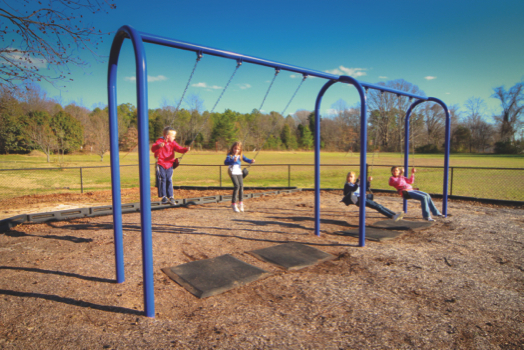
\includegraphics[width=\textwidth]{./pictures/swing-set.jpg}
\end{center}
\end{column}

\begin{column}{0.5\columnwidth}
\begin{itemize}
\item Components: chains, seats, stand structures
\item Draw a conceptual design
\item Fill a FRDPARRC sheet for each component
\item Give a safety factor + reasoning
\end{itemize}
\end{column}
\end{columns}
\end{frame}
\end{document}